\subsection{Forward charge praticle identification}
\begin{figure}[htbp]
  \centering
  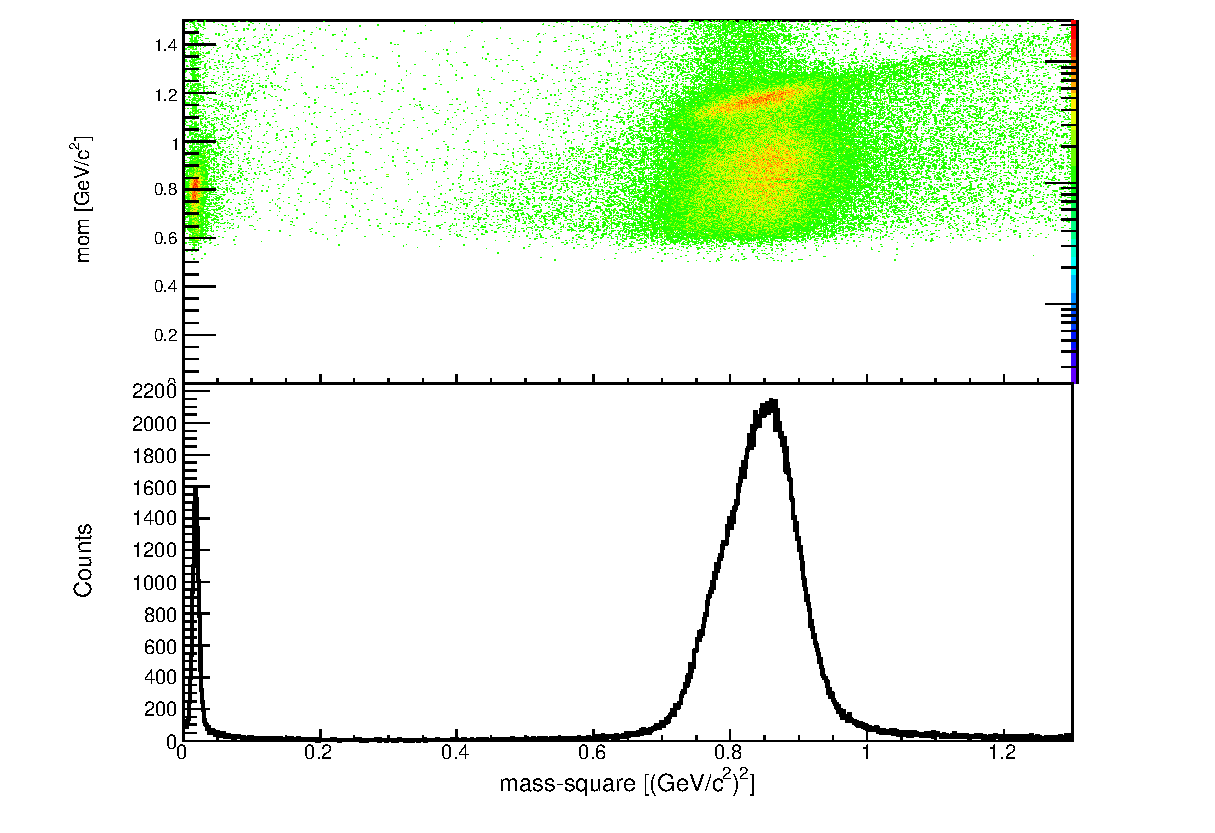
\includegraphics[width=10cm]{../pic/Dron/mass2_mom.eps}
  \caption{
    This figure shows scattered plot mass-square and momentum of forward scattered positive charged particles and horizontal axis projection (down figure).
    The $\pi^+$ peak and the proton peak were seen around $m^2 \sim 0.02 [(GeV/c^2)^2]$ and $m^2 \sim 0.85 [(GeV/c^2)^2]$, respectively.
  }
  \label{fig:FC_mass2_mom}
\end{figure}

The trajectory of the forward scattered charge particle was curve trajectory due to the Ushiwaka magnet.
The trajectory was reconstructed from the reaction vertex point, the FDC1 position, and the counter hit position using the magnetic field map of the Ushiwaka.
The field map was made by the Opera which is the software\cite{Opera} of an finite element method.
The actually used field map was scaled using the measured value at the center of Ushiwaka from the calculated map.
The trajectory of charge particle was calculated by the the third order Rungge-Kutta method and determined to minimize the weighted residual at each position.
The momentum was reconstructed from this calculation and the mass was calculated from the TOF of the T0 and the PC/CVC.
The Fig.\ref{fig:FC_mass2_mom} was shown the mass-square and the momentum as the vertical axis and the horizontal axis, respectively.
The proton peak was clearly seen in the figure, so events whose mass-square is between 0.5-2.5 $[(GeV/c^2)^2]$ were accepted as the proton.
The momentum of the proton was finally calculated using the TOF method which has higher momentum resolution than the momentum by the bending angle.
The missing mass spectrum of the $d(K^-, p)"X"$ was indicated in the Fig\ref{fig:KP_MM}.

\begin{figure}[htbp]
  \centering
  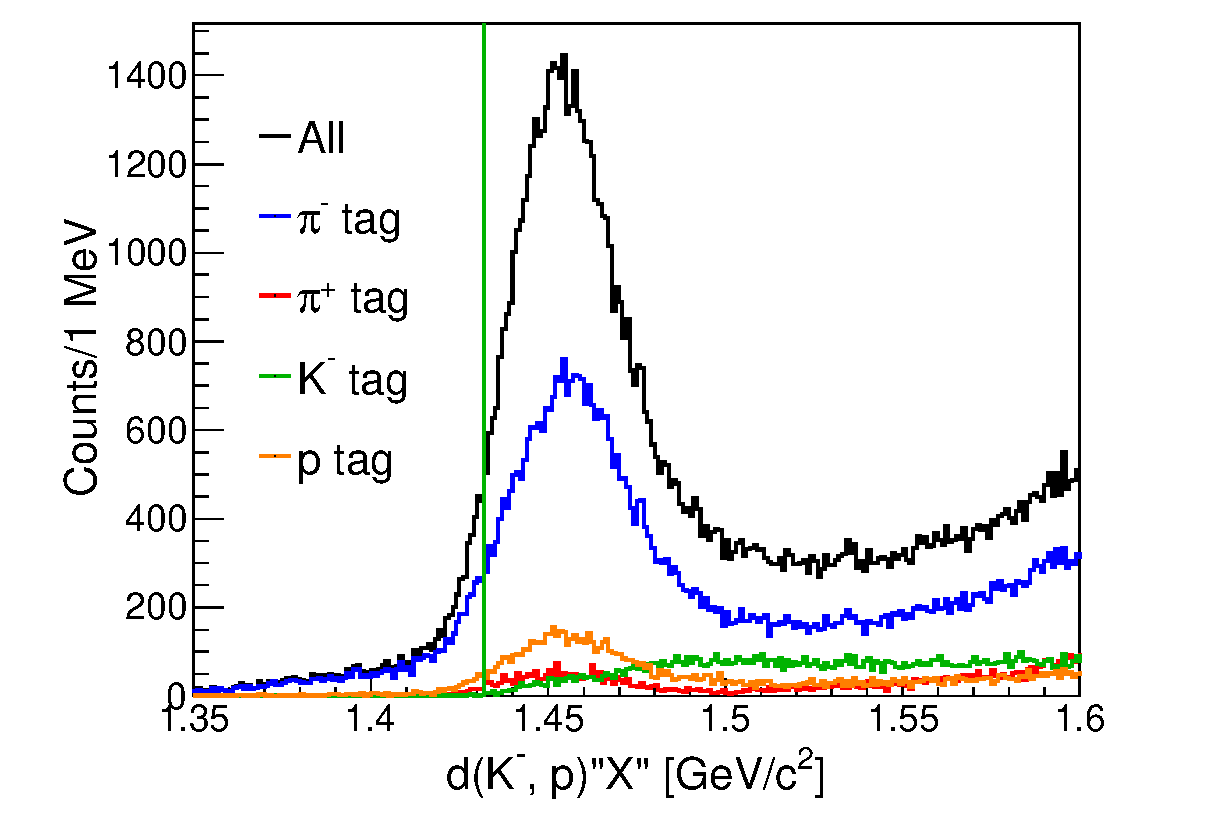
\includegraphics[width=10cm]{../pic/Run68/KP_ana/KP_MM.eps}
  \caption{
    This figure shows $d(K^-, p)"X"$ missing mass spectra.
    The black plot indicates whole data and color plots indicate CDS particles tagged data.
    These plots were adopted time offset calibration using well known particles identified by the missing mass which is described at Sec\ref{sec:KP_timeoffset}.
  }
  \label{fig:KP_MM}
\end{figure}
